%%%%%%%%%%%%%%%%%%%%%%%%%%%%%%%%%%%%%%%%%%%%%%%%%%%%%%%%%%%%%%%
%
% Welcome to Overleaf --- just edit your LaTeX on the left,
% and we'll compile it for you on the right. If you open the
% 'Share' menu, you can invite other users to edit at the same
% time. See www.overleaf.com/learn for more info. Enjoy!
%
%%%%%%%%%%%%%%%%%%%%%%%%%%%%%%%%%%%%%%%%%%%%%%%%%%%%%%%%%%%%%%%
\documentclass{beamer}
\usepackage{tikz}
\usepackage{natbib}
\usepackage{doi}
\usepackage{subcaption}
\usepackage{bibentry}

\usetheme{Frankfurt}
\usecolortheme{seahorse} 
\setbeamercolor*{item}{fg=blue}
\captionsetup{labelfont={color=blue}}
\usepackage{algorithm,algorithmic}
\setbeamertemplate{footline}[frame number]
\title{Trust Region Policy Optimization (TRPO)}
\subtitle{Original Paper by \cite{trpo_paper}}

%\title{Can we Agree to Disagree?}
\author{Matthew Vandergrift}
\institute[CMPUT 603]{Robot Learning Seminar Presentation}
\date{March 2025}

%TODO:
% add slide numbers
% 


% Testing Automated Video
\usepackage{hyperref}

% 

\begin{document}

\frame{\titlepage}

\section{Motivation}
\begin{frame}{Motivation} 
\includegraphics<1>[width=10cm,height=10cm,keepaspectratio]{Venn Diagram for Robot Learning .png}%
\includegraphics<2>[width=10cm,height=10cm,keepaspectratio]{Venn_Diagram_for_Robot_Learning _1.png}% 
\includegraphics<3>[width=10cm,height=10cm,keepaspectratio]{Venn Diagram_for_Robot_Learning_2.png}%
\end{frame}



\begin{frame}{Existing Solutions}

    \begin{itemize}
        \item Reinforce
        \item Basic Actor-Critic Algorithms 
        \item Natural Policy Gradients 
        \item Derivative Free Methods: cross-entropy method, covariance matrix adaptation. 
    \end{itemize}
    
\end{frame}

% Make this pretty, useful for introducing eta notation

\section{The Problem}
\begin{frame}{Once again, ... RL }
    "RL is computational framework for learning from interaction" \cite{rlbook}. The agent interacts with an environment with the goal of maximizing expected return. Let us denote expected return for a particular policy by $\eta(\pi)$. 

% Toss Eugene's RL interaction diagram



\end{frame}


% Building up to this Closeness Issue more mathematically 


\begin{frame}{Advantage Function}    
Recall the advantage function $A_{\pi}(s,a)$ defined as, 
\begin{equation*}
    A_{\pi}(s,a) =\  Q_{\pi}(s,a) - V_{\pi}(s)
\end{equation*}
This function tells us how "good" taking action is compared to what we would have done otherwise.
\end{frame}


\begin{frame}{Policy Improvement via Advantage}
Since policies are just collections of actions, we can use advantage function to evaluate them. Let $\pi$ and $\pi^\prime$ be two different policies. Equation $\ref{policy_a_2}$ gives a way to write the performance of $\pi^\prime$ using the performance of $\pi$ and the advantage function. 

\begin{align}
    &\eta(\pi^\prime) = \eta(\pi) + \sum_s \mu_{\pi^\prime}(s) \sum_a \pi^\prime(a \vert  s) A_{\pi}(s,a). \label{policy_a_2}
\end{align} 

Proof in appendix

\end{frame}

\begin{frame}{RL is Solved!}
At first glance we have a solution! 

\begin{algorithm}[H]
\caption{The Perfect RL Algorithm}
\begin{algorithmic}[1]
\REQUIRE $\pi$ \text{ and } $ \eta(\pi)$
\STATE $\text{max}_{\pi^\prime} \left( \eta(\pi) + \sum_s \mu_{\pi^\prime}(s) \sum_a \pi^\prime(a \vert  s) A_{\pi}(s,a) \right)$
\end{algorithmic}
\end{algorithm}

This doesn't work because we have a dependence on the policy distribution which is not something we have access to when considering $\pi^\prime$.

\end{frame}

\section{A Solution in Theory}

\begin{frame}{Dealing with $\mu_{\pi^\prime}$}

\begin{itemize}
    \item Let's use $\mu_{\pi}$ instead of $\mu_{\pi^\prime}$
    \item Define $L_{\pi}(\pi^\prime) = \eta(\pi) +  \sum_s \mu_{\pi}(s) \sum_a \pi^\prime(a \vert  s) A_{\pi}(s,a) $
    \item Assume $\pi$ is a parameterized by weights $\theta$. 
    \item Gives us a local first order approximation, $\nabla_\theta L_{\pi_{\theta_0}} (\theta_\theta) \vert_{\theta=\theta_0}  = \nabla_\theta \eta_{\pi_{\theta_0}} (\theta_\theta) \vert_{\theta=\theta_0}$
    \item If we take \textbf{small} steps in $\theta$ then we can use our 'Perfect RL algorithm'.
    % \item We have re-covered the problem Simone talked about, our approximation is only a good one local so if we move too fast things break.
\end{itemize}
\end{frame}


\begin{frame}{What is a small step?}
A Major Contribution of the Paper is the following bound, 

\begin{theorem}
Let $D_{KL}^{\text{max}}(\pi, \pi^\prime) := \text{max}_s D_{KL}\left(\pi(* \vert S) \vert\vert \pi^\prime(*\lvert s) \right).$ We then have that, 
$\eta(\pi^\prime) \geq L_{\pi}(\pi^\prime) - C D_{KL}^{\text{max}}(\pi, \pi^\prime)$ where $C = \frac{4 \epsilon \gamma}{(1-\gamma)^2}$
\end{theorem}
This  means we can bound the improvement between any-two policies based on their KL divergence. This means if we optimize within a certain KL distance we can \textit{guarantee improvement}. 
\end{frame}


% Change this title the bit might be old 
\begin{frame}{A More Perfect RL Algorithm}
    \begin{figure}
        \centering
        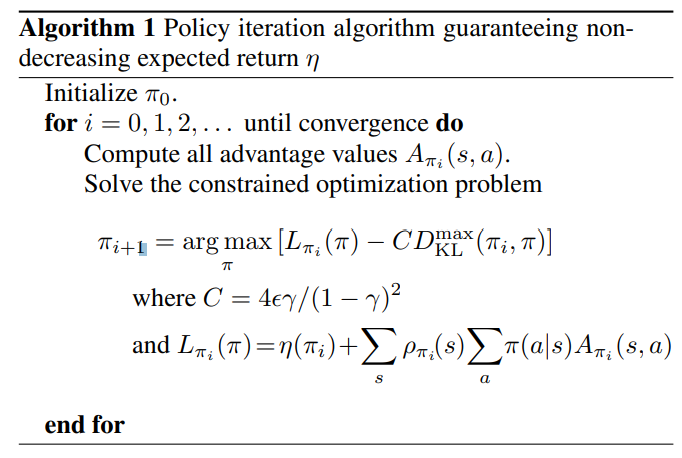
\includegraphics[width=0.7\linewidth]{TRPO_algo .png}
        \label{fig:enter-label}
    \end{figure}

The constraint is not computable due to $\text{max}_{s} f(s)$.
\end{frame}

\section{A Solution in Practice}

\begin{frame}{Make RL in Practice}
    \begin{itemize}
        \item Computable constraint 
        \vspace{4pt}
        \item Cheap cost function 
        \vspace{4pt}
        \item Cheap constrained optimization solver
    \end{itemize}
    
\end{frame}

\begin{frame}{Computable Constraint}
We want to make our constrained optimization solvable.

\begin{itemize}
    \item Get rid of max KL constraint over the whole state space. 
    \item Define 'Average' KL, $\bar{D}_{KL} := \mathbb{E}_{s \sim \mu_{\pi_{\theta}}} \left[ D_{KL}\left(\pi_{\theta}(* \vert S) \vert\vert \pi_{\theta_{old}}(*\lvert s) \right) \right] $
    \item Estimate this Expectation using roll-outs under the policy.
\end{itemize}

This gives us, 
\begin{align*}
     &\text{max}_{\theta} \hspace{5pt} L_{\theta_{old}}(\theta) \\
     &\text{subject to }  \hspace{3pt} \bar{D}_{KL}\left(\theta_{old}, \theta \right) \leq \delta
\end{align*}

%Maybe Mention, they introduce a special rollout method, but they say for phyiscal systems like Robots not to use it so I won't waste our time. 

\end{frame}

\begin{frame}{Cheap Cost Function}

We want to make $L_{\theta_{old}}(\theta)$ fast to compute. 
\begin{align*}
    & L_{\theta_{old}}(\theta) = \sum_{s} \mu_{\pi_{\theta_{old}}} \sum_a \pi_{\theta}(a \vert s) A_{\theta_{old}}(s,a) \hspace{5pt} \left(\text{Definition of $L$}\right)
    \intertext{We replace the sums by an expectation, and $A$ with estimator $\hat{A}$}
   & L_{\theta_{old}}(\theta) = \mathbb{E}_{a \sim \pi_{\theta_{old}}, s \sim \pi_{\theta_{old}}} \left[ \frac{\pi_{\theta}(a \vert s)}{\pi_{\theta_{old}}( a \vert s)} \cdot \hat{A}_{\theta_{old}}(s,a) \right] 
\end{align*}
\end{frame}


% \begin{frame}{Cheap constrained optimization solver}
%     \begin{equation*}
%         \text{max}_{\theta} \hspace{3pt} L_{\theta_{old}}(\theta) \hspace{3pt} 
%          \text{subject to }  \hspace{1pt} \bar{D}_{KL}\left(\theta_{old}, \theta \right) \leq \delta
%     \end{equation*}
    
%     We use two steps, 
%     \begin{itemize}
%         \item Compute Search Direction
%         \item Line Search in found Direction
%     \end{itemize}
    
%     \end{frame}

\begin{frame}{Cheap constrained optimization solver}
\begingroup 
\Large
\begin{equation*}
    \text{max}_{\theta} \hspace{3pt} L_{\theta_{old}}(\theta) \hspace{3pt} 
    \text{subject to }  \hspace{2pt} \bar{D}_{KL}\left(\pi_{\theta_{old}}, \pi_\theta \right) \leq \delta
\end{equation*}
\endgroup

\only<2>{\begin{figure}
    \begin{center}
        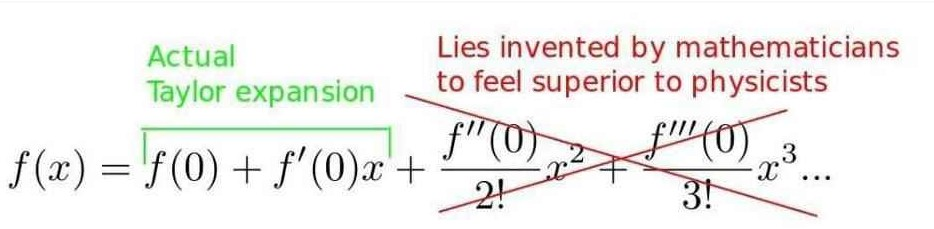
\includegraphics[width=1.1\linewidth]{20241114_122744.jpg}
        \label{fig:joke2}
    \end{center}
\end{figure}}
\end{frame}

\begin{frame}{Cheap constrained optimization solver}
    \begin{equation*}
        \text{max}_{\theta} \hspace{3pt} L_{\theta_{old}}(\theta) \hspace{3pt} 
        \text{subject to }  \hspace{2pt} \bar{D}_{KL}\left(\pi_{\theta_{old}}, \pi_\theta \right) \leq \delta
    \end{equation*}
\only<1->{First Order of Taylor Expansion to $L_{\theta_{old}}(\theta)$}    
\only<2->{\begin{align*} 
    \only<2->{& L_{\theta_{old}}(\theta) \approx L_{\theta_{old}}(\theta_{old}) + g^T (\theta - \theta_{old})} \\ 
    \only<3->{& L_{\theta_{old}}(\theta) \approx 0 + g^T (\theta - \theta_{old})} 
    \only<4->{\intertext{Let $\Delta \theta = (\theta - \theta_{old}) $}}
    \only<5->{& L_{\theta_{old}}(\theta) \approx g^T \Delta\theta} 
\end{align*}}
\end{frame}


\begin{frame}{Cheap constrained optimization solvers}
    \begin{equation*}
                \text{max}_{\theta} \hspace{3pt} L_{\theta_{old}}(\theta) \hspace{3pt} 
                 \text{subject to }  \hspace{1pt} \bar{D}_{KL}\left(\pi_{\theta_{old}}, \pi_\theta \right) \leq \delta
        \end{equation*}
    
    \only<1->{Second Order of Taylor Expansion of Contraint}    
    \only<2>{\begin{align*} 
        \only<2->{& \bar{D}_{KL}\left(\pi_{\theta_{old}}, \pi_{\theta} \right) \approx \bar{D}_{KL}\left(\pi_{\theta_{old}}, \pi_{\theta_{old}} \right)  + \nabla_{\theta} \hat{D}_{KL} (pi_{\theta_{old}} \vert\vert \pi_\theta)\vert_{\theta_{old}} \cdot(\theta - \theta_{old}) + \\
        \only<3->{& \hspace{15pt} \frac{1}{2}(\theta - \theta_{old})^TH(\theta - \theta_{old})}} \\
        \only<4->{& \bar{D}_{KL}\left(\pi_{\theta_{old}}, \pi_{\theta} \right) \approx 0 + 0 + \frac{1}{2}\Delta\theta ^TH\Delta\theta} \\ 
        only<5->{& \bar{D}_{KL}\left(\pi_{\theta_{old}}, \pi_{\theta} \right) \approx  \frac{1}{2}\Delta\theta ^TH\Delta\theta}
    \end{align*}}
\end{frame}

\begin{frame}{Cheap constrained optimization solvers}
    We now have a new constrained optimization problem, 
    \begin{align*}
        & \text{argmax}_{\theta}\hspace{4pt} g^T \Delta\theta   \\
        & \text{subject to  } \frac{1}{2}\Delta\theta ^TH\Delta\theta \leq \delta
    \end{align*}
Now since it's a nice quadratic/convex contrainst we can solve, 

\begin{equation*}
    \theta = \theta_{old} + \sqrt{\frac{2\delta}{g^tH^{-1}g}} H^{-1}g. 
\end{equation*}
\hyperlink{done_deriv}{\beamerbutton{skip derivation}}
\end{frame}

\begin{frame}{Steps to Solve}
    \vspace{-20.5pt}
    \begin{align*}
        & \text{argmax}_{\theta}\hspace{4pt} g^T \Delta\theta \hspace{10pt} \text{subject to  } \frac{1}{2}\Delta\theta ^TH\Delta\theta \leq \delta
    \end{align*}
    \vspace{-45.5pt}
    \begin{align*}
        \only<1->{\intertext{Use Lagrangian to solve the constrained optimization}} 
        \only<2->{& L = g^T\Delta\theta + \lambda \left( \frac{1}{2}(\theta - \theta_{old})^TH(\theta - \theta_{old}) - \delta \right)} \\ 
        \only<3->{& \nabla_{\theta} L = 0 \implies g^T + \frac{\lambda}{2} H\Delta\theta = 0 } \\
        \only<4->{& \Delta\theta =  -\frac{2}{\lambda}H^{-1}g} 
        \only<5->{\intertext{ This looks like SGD, set $\alpha = -\frac{2}{\lambda}$}} 
        \only<6->{& \Delta\theta =  \alpha H^{-1}g}
    \end{align*} 
\end{frame}

\begin{frame}{Steps to Solve}
    \vspace{-35.5pt}
    \begin{align*}
        \only<1->{\intertext{We have $\Delta\theta = \alpha H^{-1}g$, and we solve for $\alpha$ by setting contraint $=\delta$}}
        \only<2->{& \frac{1}{2}\Delta\theta ^TH\Delta\theta = \delta}  \\
        \only<3->{& \frac{1}{2}  \alpha H^{-1}g^T H \alpha H^{-1}g  = \delta} 
        \only<4->{\intertext{Now we simply re-arrange}}
        \only<5->{& \alpha^2 g^THg = 2\delta} \\
        \only<6->{& \alpha = \sqrt{\frac{2\delta}{g^tHg}}} 
        \only<7->{& \intertext{Subbing this into $\Delta\theta = \theta - \theta_{old} = \alpha H^{-1}g$ we get}}
        \only<8->{& \theta = \theta_{old} + \sqrt{\frac{2\delta}{g^THg}}H^{-1}g}
    \end{align*}
\end{frame}


\begin{frame}{$H^{-1}g$}
\label{done_deriv}

\begin{figure}
    \centering
    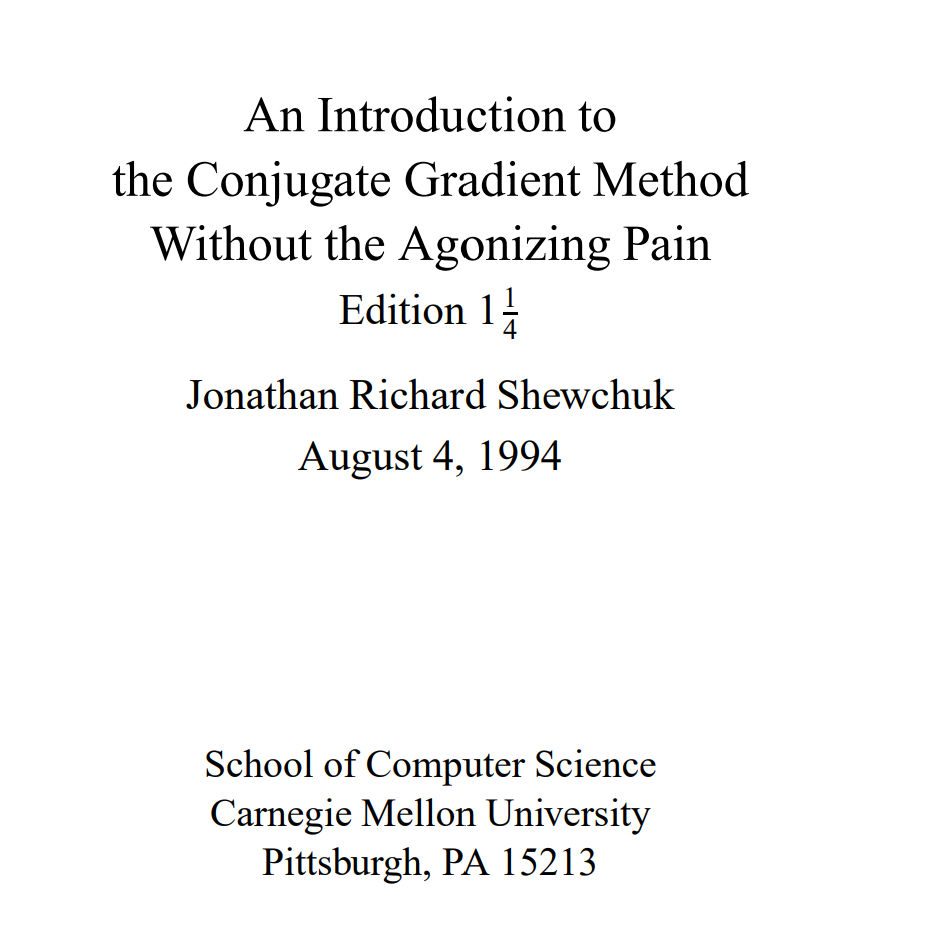
\includegraphics[width=1.1\linewidth]{trpo_funny_reference.png}
    \label{fig:joke}
\end{figure}    
\end{frame}

\begin{frame}{Line Search}
    Our approximations have gone back to bite us. We need to check that our ubdpates don't exceed our \textit{actual} constraint using a line search. 
\end{frame}


\begin{frame}{Trust Region Policy Optimization}
    
    \begin{figure}
        \centering
        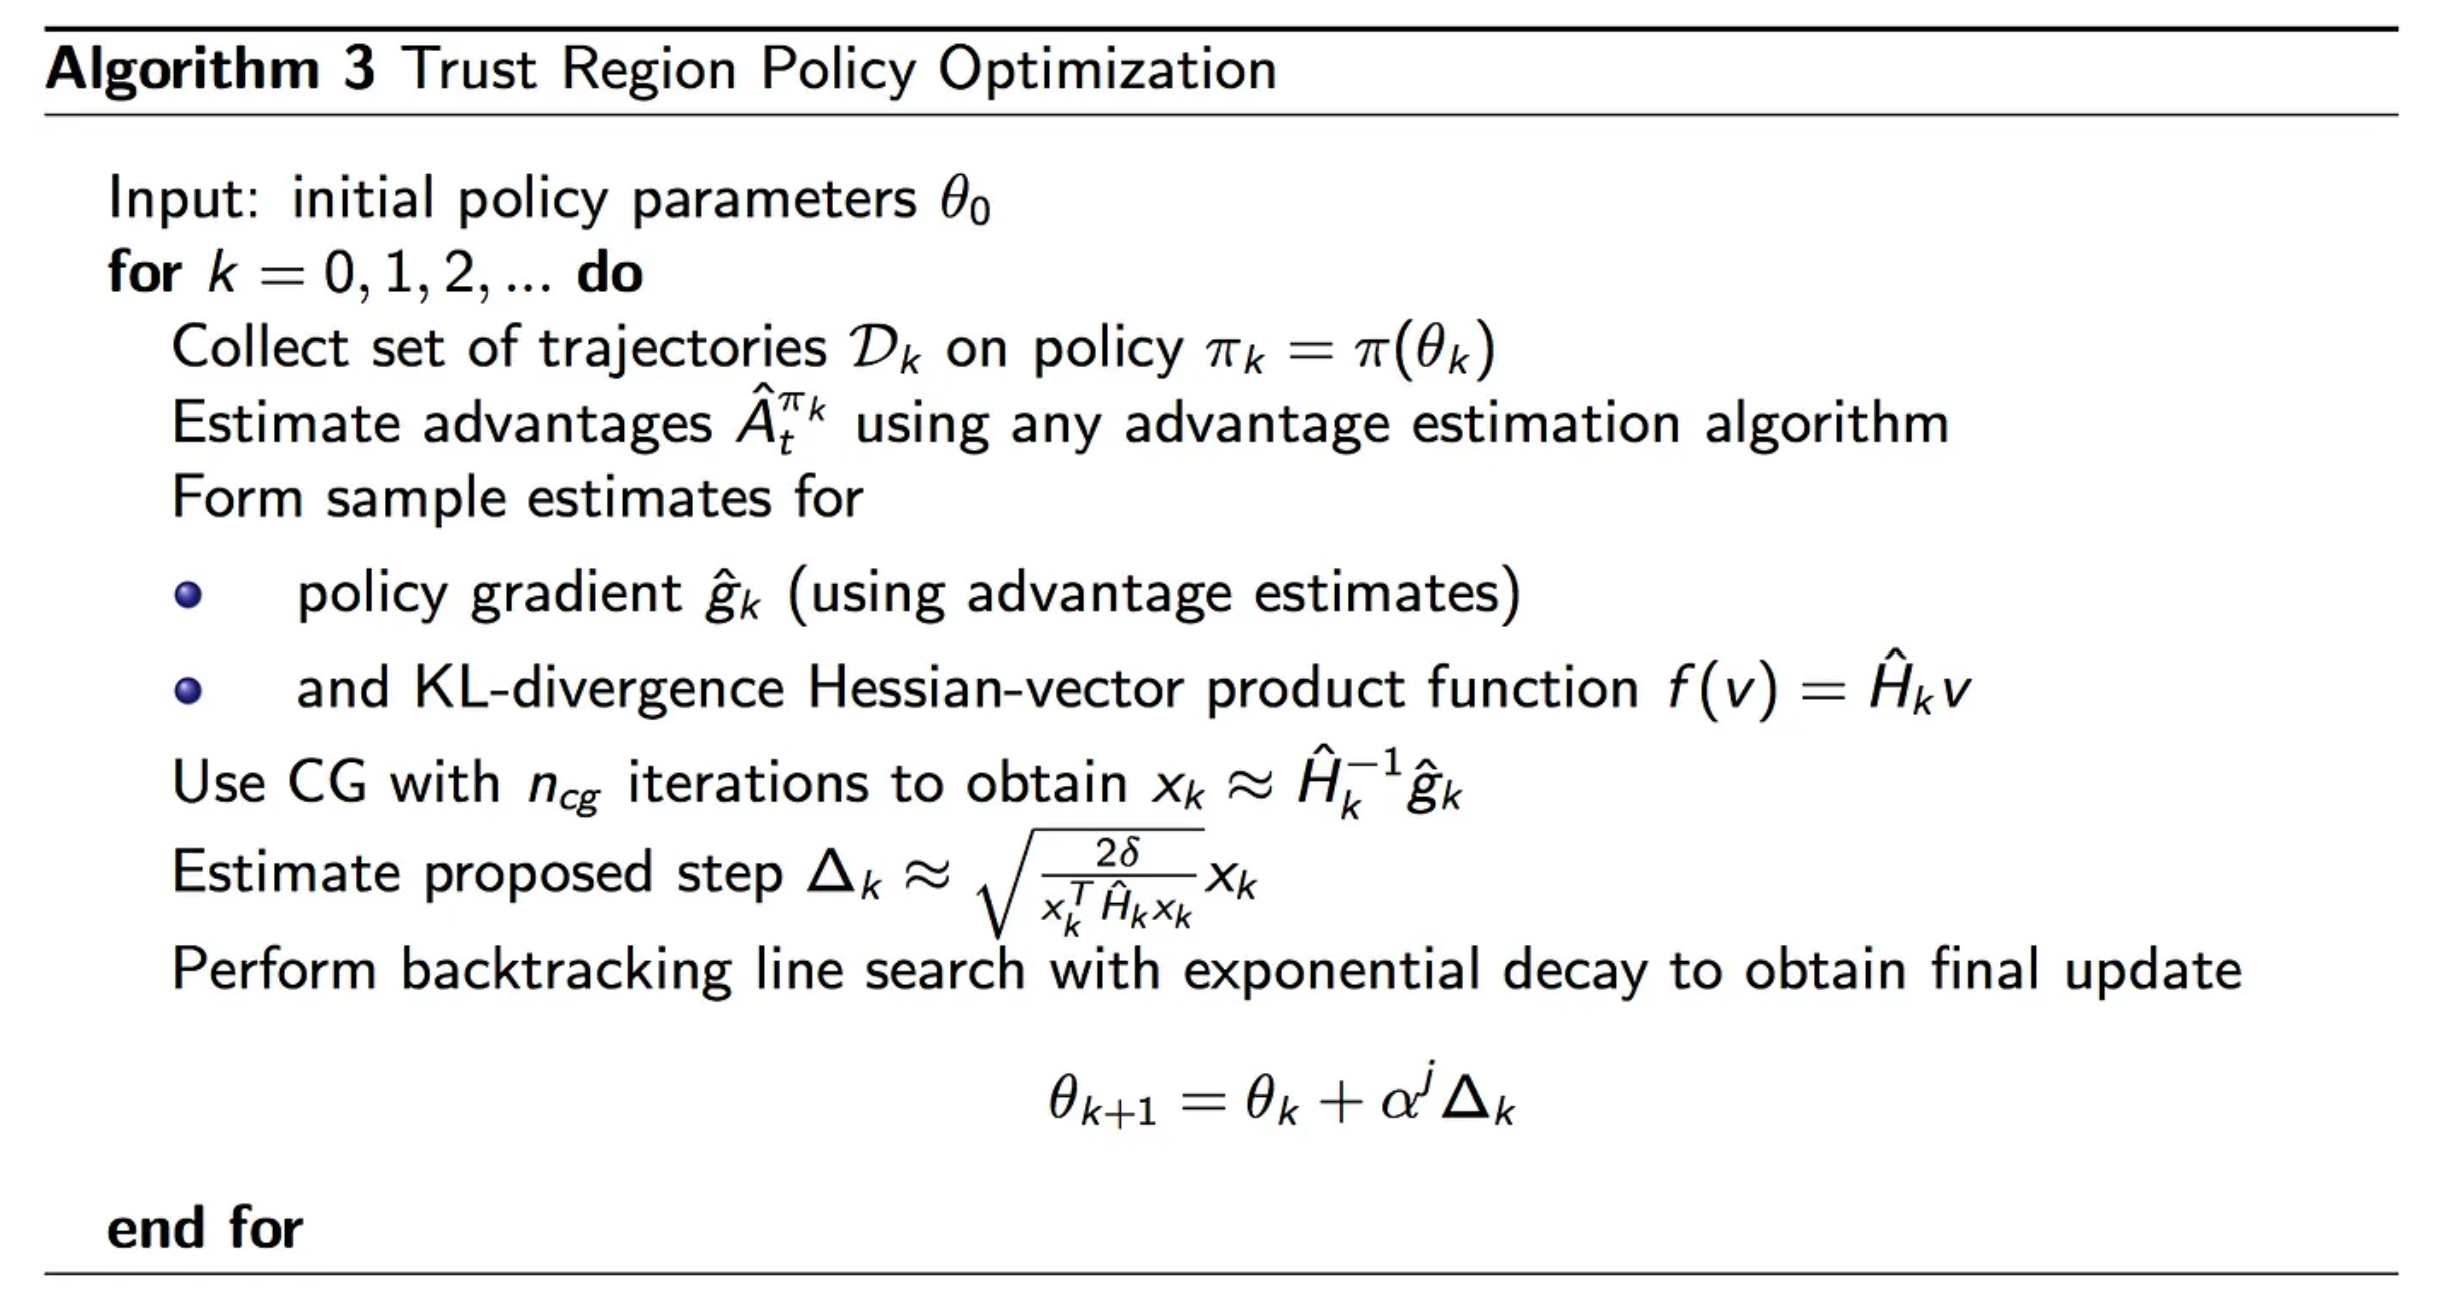
\includegraphics[width=1\linewidth]{trpo_algorithm_pseudocode.png}
        \label{fig:algo_pseudocode}
    \end{figure}    

    
\end{frame}

\section{TRPO for Robot Learning}
\begin{frame}{Experimental Results in TRPO Paper}    

\begin{figure}
    \centering
    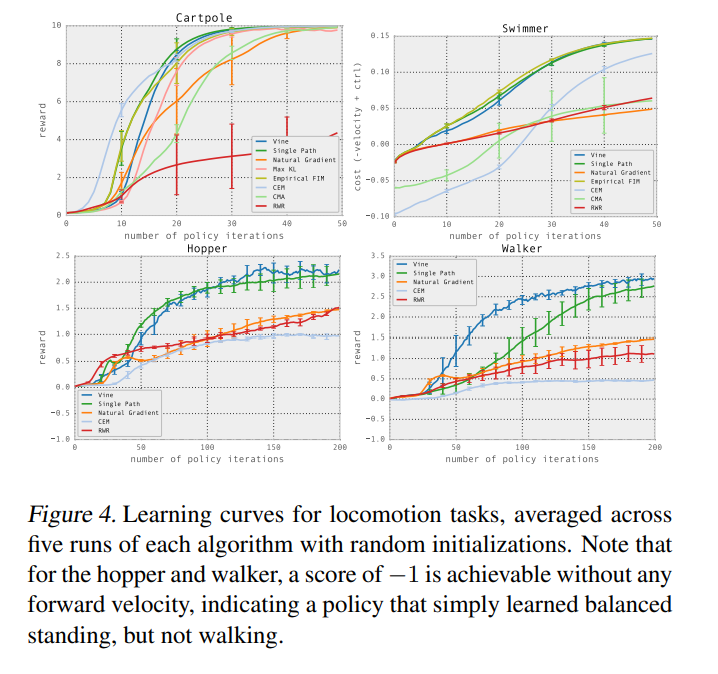
\includegraphics[width=0.8\linewidth]{trpo_experimental_results.png}
    \label{fig:exp_results}
\end{figure}


\end{frame}

\begin{frame}{External TRPO Robotics Applications}    

\cite{benchmark_robots} wrote a paper bencmarking policy gradient algorithms for robotics, including TRPO. 
\begin{itemize}
    \item "TRPO achieving near-best final learning performance in all tasks." 
    \item "Among these algorithms, the final performance of TRPO was never substantially worse compared to the best in each task."
    \item  "TRPO’s performance was the least sensitive to hyper-parameter variations with the smallest interquartile range on both tasks."
\end{itemize}

\end{frame}

\begin{frame}{Next Steps}
    \begin{itemize}
        \item The Chosen Path
        \begin{itemize}
            \item Clipping
            \item Hyperparameter tuning
        \end{itemize}
        \vspace{10pt}
        \item Other Approaches:
        \begin{itemize}
            \item More precise approximations $\rightarrow$ no more line search
            \item Assumptions about policy structure $\rightarrow$ tighter bound 
            \item Assumptions about function approximator $\rightarrow$ better notation of small step
        \end{itemize}
    \end{itemize}

\end{frame}

\newcommand{\bluecheck}{}%
\DeclareRobustCommand{\greencheck}{%
  \tikz\fill[scale=0.4, color=green]
  (0,.35) -- (.25,0) -- (1,.7) -- (.25,.15) -- cycle;%
}
\newcommand{\tikzxmark}{%
\tikz[scale=0.23, color=red] {
    \draw[line width=0.7,line cap=round] (0,0) to [bend left=6] (1,1);
    \draw[line width=0.7,line cap=round] (0.2,0.95) to [bend right=3] (0.8,0.05);
}}



\begin{frame}{Critiques of the Paper}
   
    %\scalebox{1.5}{TLDR : Content: \greencheck \hspace{4pt} Presentation \tikzxmark}
    \begin{itemize}
        \item They leave out critical implementation details \citep{deepRL_matters}. 
        \item They compare 'Vine' and 'Path', and Vine is a different problem formulation 
        %\item  \href{https://jonathan-hui.medium.com/rl-trust-region-policy-optimization-trpo-part-2-f51e3b2e373a}{TRPO-Blog for Details}
    \end{itemize}

\begin{figure}
    \centering
    \includegraphics[width=0.7\linewidth]{TRPO_Issues.png}
    \label{fig:issues}
\end{figure}

\end{frame}


\begin{frame}{Thank you for listening}

\href{https://www.youtube.com/watch?v=ovDfhvjpQd8&t=387s}{Robots following TRPO Policies}

\end{frame}




\begin{frame}{References}
    \bibliographystyle{plainnat}
    \bibliography{references}
\end{frame}


\end{document}